%%%%%%%%%%%%%%%%%%%%%%%%%%%%%%%%%%%%%%%%%
% Beamer Presentation
% LaTeX Template
% Version 1.0 (10/11/12)
%
% This template has been downloaded from:
% http://www.LaTeXTemplates.com
%
% License:
% CC BY-NC-SA 3.0 (http://creativecommons.org/licenses/by-nc-sa/3.0/)
%
%%%%%%%%%%%%%%%%%%%%%%%%%%%%%%%%%%%%%%%%%

%----------------------------------------------------------------------------------------
%	PACKAGES AND THEMES
%----------------------------------------------------------------------------------------

\documentclass{beamer}

\mode<presentation> {

% The Beamer class comes with a number of default slide themes
% which change the colors and layouts of slides. Below this is a list
% of all the themes, uncomment each in turn to see what they look like.

%\usetheme{default}
%\usetheme{AnnArbor}
%\usetheme{Antibes}
%\usetheme{Bergen}
%\usetheme{Berkeley}
%\usetheme{Berlin}
%\usetheme{Boadilla}
%\usetheme{CambridgeUS}
%\usetheme{Copenhagen}
%\usetheme{Darmstadt}
%\usetheme{Dresden}
%\usetheme{Frankfurt}
%\usetheme{Goettingen}
%\usetheme{Hannover}
%\usetheme{Ilmenau}
%\usetheme{JuanLesPins}
%\usetheme{Luebeck}
\usetheme{Madrid}
%\usetheme{Malmoe}
%\usetheme{Marburg}
%\usetheme{Montpellier}
%\usetheme{PaloAlto}
%\usetheme{Pittsburgh}
%\usetheme{Rochester}
%\usetheme{Singapore}
%\usetheme{Szeged}
%\usetheme{Warsaw}

% As well as themes, the Beamer class has a number of color themes
% for any slide theme. Uncomment each of these in turn to see how it
% changes the colors of your current slide theme.

%\usecolortheme{albatross}
%\usecolortheme{beaver}
%\usecolortheme{beetle}
%\usecolortheme{crane}
%\usecolortheme{dolphin}
%\usecolortheme{dove}
%\usecolortheme{fly}
%\usecolortheme{lily}
%\usecolortheme{orchid}
%\usecolortheme{rose}
%\usecolortheme{seagull}
%\usecolortheme{seahorse}
%\usecolortheme{whale}
%\usecolortheme{wolverine}

%\setbeamertemplate{footline} % To remove the footer line in all slides uncomment this line
%\setbeamertemplate{footline}[page number] % To replace the footer line in all slides with a simple slide count uncomment this line

%\setbeamertemplate{navigation symbols}{} % To remove the navigation symbols from the bottom of all slides uncomment this line
}

\usepackage[english,spanish]{babel}
\usepackage{graphicx} % Allows including images
\usepackage{booktabs} % Allows the use of \toprule, \midrule and \bottomrule in tables
\usepackage{subfig}
\usepackage[export]{adjustbox}

%----------------------------------------------------------------------------------------
%	TITLE PAGE
%----------------------------------------------------------------------------------------

\title[Clasificación de imágenes médicas]{Análisis y clasificación de imágenes médicas mediante redes neuronales} % The short title appears at the bottom of every slide, the full title is only on the title page

\author{Gonzalo Caparrós Laiz} % Your name
\institute[UM] % Your institution as it will appear on the bottom of every slide, may be shorthand to save space
{
Universidad de Murcia \\ % Your institution for the title page
\medskip
\textit{gonzalo.caparrosl@um.es} % Your email address
}
\date{Junio, 2020} % Date, can be changed to a custom date

\begin{document}

\begin{frame}
\titlepage % Print the title page as the first slide
\end{frame}

%\begin{frame}
%\frametitle{Índice} % Table of contents slide, comment this block out to remove it
%\tableofcontents % Throughout your presentation, if you choose to use \section{} and \subsection{} commands, these will automatically be printed on this slide as an overview of your presentation
%\end{frame}

%----------------------------------------------------------------------------------------
%	PRESENTATION SLIDES
%----------------------------------------------------------------------------------------

\begin{frame}
\frametitle{Inteligencia Artificial}

\begin{block}{Inteligencia Artificial}
Programas que intentan simular el comportamiento humano para resolver un problema.
\end{block}

\begin{itemize}
\item Machine learning: es un tipo de inteligencia artificial, al algoritmo no se le especifica cómo resolver la tarea, sino que el algoritmo aprende.
\begin{itemize}
\item Aprendizaje supervisado: datos de entrada etiquetados.
\item Aprendizaje no supervisado: datos de entrada no etiquetados.
\item Aprendizaje por refuerzo: la entrada es lo que perciben los agentes.
\end{itemize}
\item Redes Neuronales: es un tipo de machine learning, se organiza en capas de neuronas que se interconectan.
\end{itemize}

\end{frame}



\begin{frame}
\frametitle{Tipos de capas}

\begin{itemize}
\setlength\itemsep{1em}
\item Totalmente conectada: neuronas conectadas todas con todas.
\item Convolución: combina un grupo de salidas de la capa anterior en uno.
\item Convolución dilatada: similar a la convolución, entrada dispersa.
\end{itemize}

\begin{block}{Concatenación, pool, dropout y softmax}
No hacen tienen la función de aprender pero, hacen diferentes funciones: agrupar, reducir tamaño, modificar valores aleatorios y redistribuir la salida.
\end{block}

\end{frame}



\begin{frame}
\frametitle{Técnicas}

\begin{itemize}
\setlength\itemsep{1em}
\item Transfer learning: partir de una red neuronal entrenada y eliminar las últimas capas para reentrenarlas.
\item Random forest: dividir la tarea principal en varios subtareas más simples y construir un árbol de decisión.
\item Cascada: organizar una serie de modelos en secuencia, cada uno confirma o descarta una clase.
\end{itemize}

\end{frame}



\begin{frame}
\frametitle{Entrada de datos}

\begin{itemize}
\item Características deseables dataset:
\begin{itemize}
\item Misma proporción.
\item Mantener la proporción al hacer la división.
\item Tener en cuenta los datos relacionados a la hora de dividir el dataset.
\end{itemize}
\end{itemize}

\begin{block}{Distorsión}
Aplicar algunas transformaciones al conjunto de datos de entrada.
\begin{itemize}
\item Aumentar el tamaño del conjunto de datos de entrada.
\item Mejorar la calidad de un conjunto de datos.
\end{itemize}
\end{block}

\end{frame}



\begin{frame}
\frametitle{Bottleneck}

Dividir el entrenamiento en dos pasos: primero obtener los valores del \textit{tensor} de salida de todo el dataset y después entrenar las ultimas capas usando como entrada los valores obtenidos.

\begin{figure}[H]
\centering
\subfloat[Entrenamiento]{{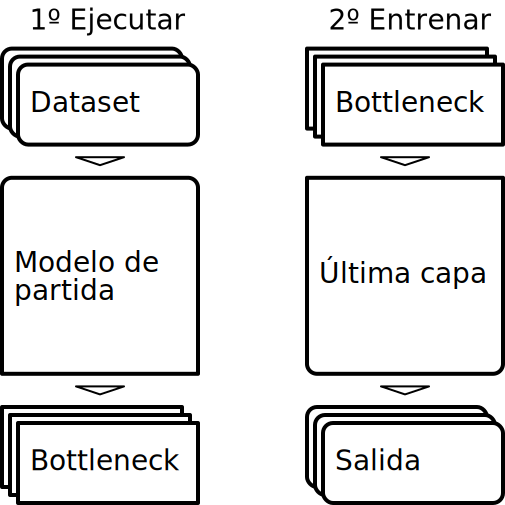
\includegraphics[valign=c, width=0.3\textwidth]{img/entrenamiento_bottleneck} }}%
\qquad
\subfloat[Inferencia]{{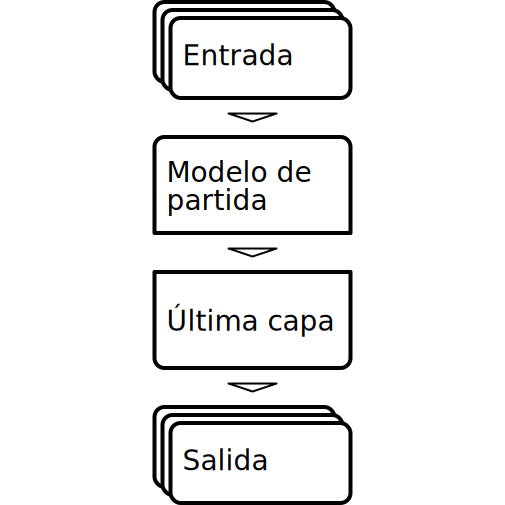
\includegraphics[valign=c, width=0.3\textwidth]{img/inferencia_bottleneck} }}%
\caption{Pasos para realizar el entrenamiento usando la técnica de \textit{bottleneck} y para la inferencia.}
\end{figure}

\end{frame}



\begin{frame}
\frametitle{Entrenamiento completo}

En esta prueba se entrena de 0 la arquitectura \textit{AlexNet} para clasificar las imágenes del \textit{dataset} \textit{cifar 10}.

\begin{table}[H]
\centering
\resizebox{\textwidth}{!}{%
\begin{tabular}{|l|l|l|l|l|l|l|}
\hline
\textbf{Modelo} & \textbf{Dataset}              & \textbf{Clases}         & \textbf{Iteraciones}        & \textbf{Learning rate}   & \textbf{Batch size}      & \textbf{Precisión}        \\ \hline
AlexNet         & \multicolumn{1}{c|}{cifar 10} & \multicolumn{1}{c|}{10} & \multicolumn{1}{c|}{100000} & \multicolumn{1}{c|}{0.1} & \multicolumn{1}{c|}{128} & \multicolumn{1}{c|}{86.0} \\ \hline
\end{tabular}%
}
\caption{Resultado entrenamiento completo.}
\end{table}

En esta prueba se obtiene un 86\% de precisión, que es un buen resultado para la prueba que se ha realizado, un entrenamiento completo. De esta forma se ha entrenado un modelo específicamente para ese \textit{dataset}.

\end{frame}



\begin{frame}
\frametitle{Añadir una capa}

\begin{table}[H]
\centering
\resizebox{\textwidth}{!}{%
\begin{tabular}{|l|l|c|c|c|c|c|}
\hline
\textbf{Modelo} & \textbf{Dataset}                                                  & \textbf{Clases} & \textbf{Iteraciones} & \textbf{Learning rate} & \textbf{Batch size} & \textbf{Precisión} \\ \hline
inception v3    & \begin{tabular}[c]{@{}l@{}}subconjunto\\ de cifar 10\end{tabular} & 3               & 4000                 & 0.01                   & 100                 & 93.8               \\ \hline
inception v3    & flores                                                            & 5               & 4000                 & 0.01                   & 100                 & 90.9               \\ \hline
inception v3    & cifar 10                                                          & 10              & 4000                 & 0.01                   & 100                 & 79.5               \\ \hline
inception v3    & cifar 100                                                         & 20              & 4000                 & 0.01                   & 100                 & 64.1               \\ \hline
inception v3    & cifar 100                                                         & 100             & 4000                 & 0.01                   & 100                 & 51.7               \\ \hline
resnet v2 152   & \begin{tabular}[c]{@{}l@{}}subconjunto\\ de cifar 10\end{tabular} & 3               & 4000                 & 0.01                   & 100                 & 94.4               \\ \hline
resnet v2 152   & cifar 10                                                          & 10              & 40000                & 0.01                   & 100                 & 82.9               \\ \hline
resnet v2 152   & cifar 100                                                         & 20              & 14000                & 0.01                   & 100                 & 70.8               \\ \hline
\end{tabular}%
}
\caption{Resultados añadir una capa totalmente conectada y \textit{softmax}.}
\end{table}

\end{frame}



\begin{frame}
\frametitle{Añadir y quitar capas}

\begin{table}[H]
\centering
\resizebox{\textwidth}{!}{%
\begin{tabular}{|l|l|c|c|c|c|c|}
\hline
\textbf{Modelo} & \textbf{Dataset} & \textbf{Clases} & \textbf{Iteraciones} & \textbf{Learning rate} & \textbf{Batch size} & \textbf{Precisión} \\ \hline
inception + 3 capas    & cifar 10         & 10              & 4000                 & 0.01                   & 100                 & 34.1               \\ \hline
inception + 3 capas    & cifar 10         & 10              & 50000                & 0.01                   & 100                 & 79.9               \\ \hline
inception + 3 capas    & cifar 100        & 100             & 60000                & 0.01                   & 100                 & 45.5               \\ \hline
inception - 2 capas    & cifar 10                                                          & 10              & 100000               & 0.01                   & 100                 & 79.8               \\ \hline
inception - 2 capas    & \begin{tabular}[c]{@{}l@{}}subconjunto\\ de cifar 10\end{tabular} & 3               & 70000                & 0.01                   & 100                 & 95.5               \\ \hline
inception - 3 capas    & cifar 10                                                          & 10              & 90000                & 0.01                   & 100                 & 56.0               \\ \hline
inception - 3 capas    & \begin{tabular}[c]{@{}l@{}}subconjunto\\ de cifar 10\end{tabular} & 3               & 70000                & 0.01                   & 100                 & 95.9               \\ \hline
\end{tabular}%
}
\caption{Resultados añadir y quitar capas.}
\end{table}

\end{frame}



\begin{frame}
\frametitle{Añadir una capa}
Añadir una capa pero bien

\end{frame}



\begin{frame}
\frametitle{Usar un slice}

\end{frame}



\begin{frame}
\frametitle{Cascada}
Subsets

\end{frame}



\begin{frame}
\frametitle{Resultados cascada}

\end{frame}



\begin{frame}
\frametitle{Inferencia por paciente}

\end{frame}



\begin{frame}
\frametitle{Distorsión}

\end{frame}



\begin{frame}
\frametitle{Resultado final}

\end{frame}



\begin{frame}
\frametitle{Vías futuras}

\end{frame}



\begin{frame}
\Huge{\centerline{Fin}}
\end{frame}

\end{document} 